Für den Client wird eine graphische Benutzerschnittstelle gewählt.
Eine solche bietet dem Benutzer eine einfache Bedienung und ermöglicht es komplexe Zusammenhänge einfach für den Spieler darzustellen.
Des weiteren bietet eine graphische Benutzerschnittstelle mehr Möglichkeiten, wie der Spieler mit dem Spiel interagieren kann als eine Kommanozeilenanwendung.\\

Im folgenden werden die einzelnen Dialoge und Popups aufgelistet und welche Anwendungsfälle diese jeweils abdecken

\begin{itemize}
	\item Dialog Hauptmenü: Hauptmenü anzeigen, Anwendung beenden, zur Lobbyübersicht wechseln, Einstellungen, Hilfe anzeigen
	\item Dialog Einstellungen: Vornehmen von Einstellungen
	\item Popup Hilfe: Anzeigen von Hilfsfunktionen
	\item Popup Fehler bei der Verbindung zum Server: Übergang zur Lobbyübersicht, Fehlerfall
	\item Dialog Lobbyübersicht: Lobbyübersicht anzeigen, Lobbyübersicht verlassen, Lobby erstellen, Lobby beitreten, Nutzernamen festlegen
	\item Popup Nutzernamen ändern: Nutzernamen festlegen
	\item Popup Lobbyname eingeben und Konfig. erstellen: Konfigurationsdaten festlegen
	\item Dialog Editor: erstellen von Konfigurationsdaten
	\item Dialog Lobby: Lobby anzeigen
	\item Popup Rolle ändern: Rolle wechseln
	\item Popup Konfiguration anzeigen: anzeigen der Konfiguration
	\item Dialog Wahlphase: Wahlphase anzeigen, Character/Gadget wählen
	\item Dialog Ausrüstungsphase: Ausrüstungsphase anzeigen, Gadget zuweisen
	\item Dialog Spielbildschirm: Spielbildschirm anzeigen, Spielstand darstellen, Spielaktion durchführen, Spiel verlassen
	\item Popup Optionen: Einstellungen, Spiel pausieren
	\item Popup Einstellungen: Einstellungen vornehmen
	\item Popup Pausieren: Spiel pausieren und entpausieren
	\item Dialog Gewinnerbildschirm: Gewinnerbildschirm anzeigen, Gewinner zeigen, Statistiken anzeigen
\end{itemize}

Im Spielbildschirm wurden alle möglichen Aktionen die ein Spieler durchführen kann aus Übersichtlichkeitsgründen zu \textit{Spielaktion durchführen} zusammengefasst. Dazu gehören Charakter anzeigen, Feld anzeigen, Charakter bewegen, Gadget verwenden, etc.
\begin{figure}
  \centering
  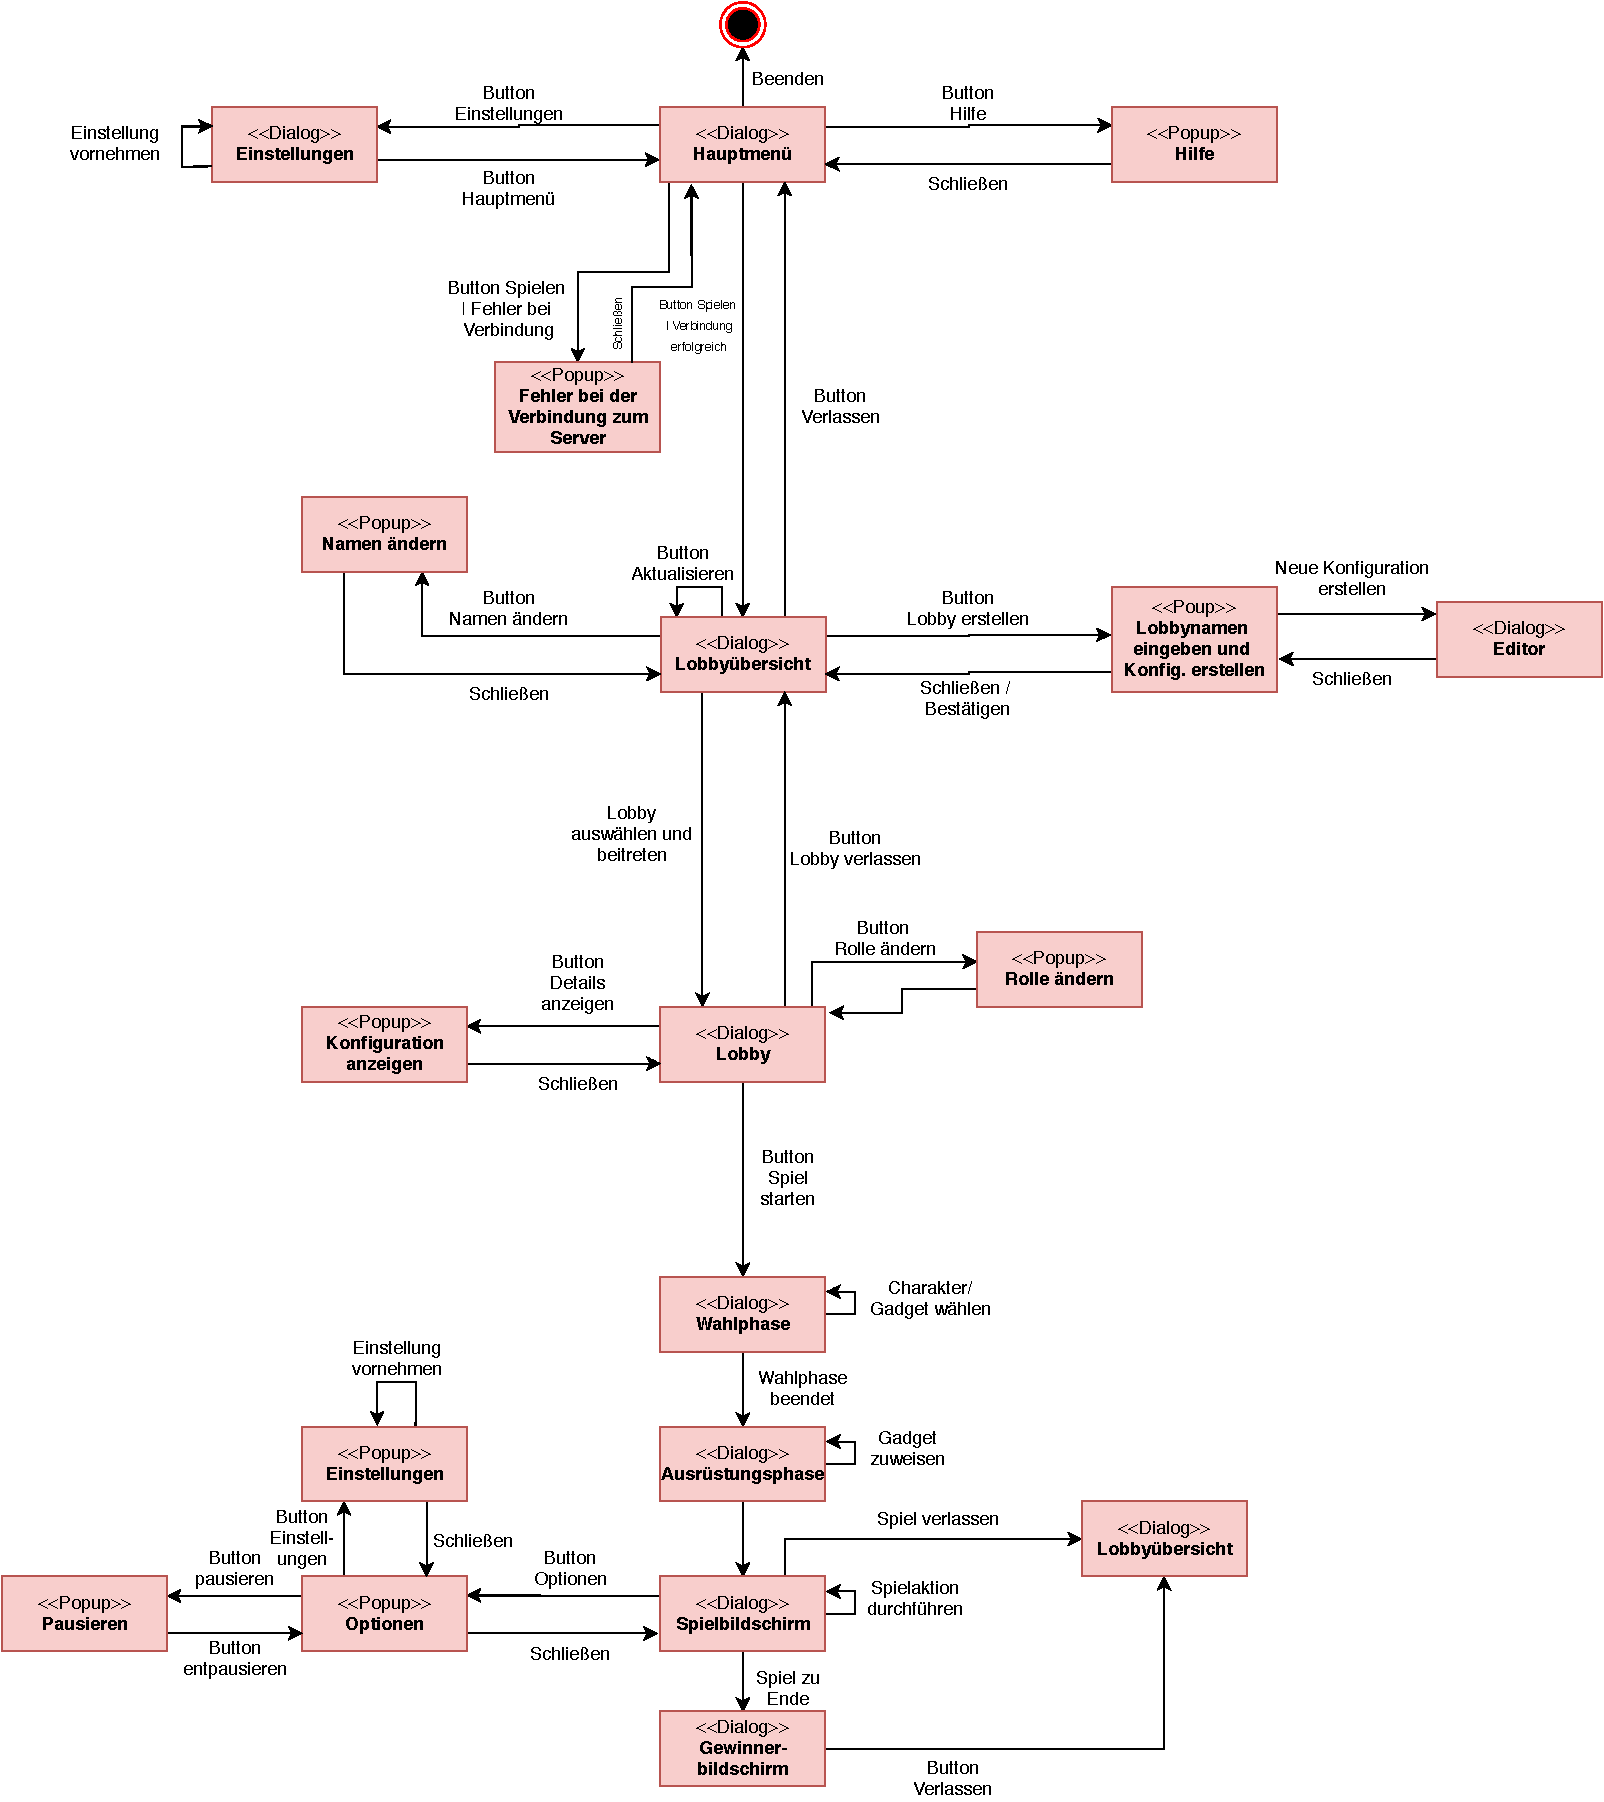
\includegraphics[width=\textwidth]{Meilenstein03/client_dialog.pdf}
  \caption{Dialog Diagram für den Client}
\end{figure}
